\documentclass[tikz,border=2pt]{standalone}
\usepackage{amsmath}
\usetikzlibrary{arrows.meta}
\begin{document}
% for (i in x) s <- s + i with x = 1:6: one pass per element; the accumulator s goes
% 0, 1, 3, 6, 10, 15, 21, which equals sum(x).
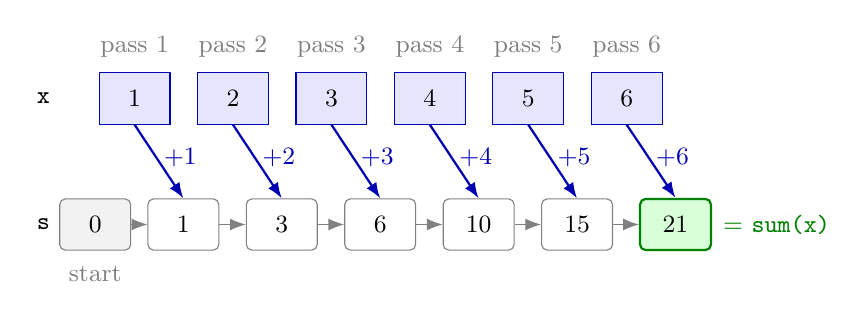
\begin{tikzpicture}[font=\small, >={Latex[length=2mm]},
  cell/.style={draw=blue!70!black, fill=blue!10, minimum width=9mm, minimum height=6.5mm},
  acc/.style={draw=gray, rounded corners=2pt, minimum width=9mm, minimum height=6.5mm}]
  \node[anchor=east] at (0.3,0) {\texttt{x}};
  \node[anchor=east] at (0.3,-1.6) {\texttt{s}};
  \foreach \v [count=\k] in {1,2,3,4,5,6} {
    \node[cell] (c\k) at (1.25*\k,0) {\v};
    \node[gray] at (1.25*\k,0.65) {pass \k};
  }
  \node[acc, fill=gray!10] (s0) at (0.75,-1.6) {0};
  \foreach \s [count=\k] in {1,3,6,10,15} {
    \node[acc] (s\k) at (1.25*\k+0.62,-1.6) {\s};
  }
  \node[acc, draw=green!50!black, fill=green!15, thick] (s6) at (1.25*6+0.62,-1.6) {21};
  \foreach \k [evaluate=\k as \j using int(\k-1)] in {1,...,6} {
    \draw[->, thin, gray] (s\j) -- (s\k);
    \draw[->, thick, blue!70!black] (c\k.south) -- node[pos=0.45, right=-1pt, font=\small, blue!70!black] {$+\k$} (s\k.north);
  }
  \node[anchor=west, green!50!black] at (8.6,-1.6) {$=$ \texttt{sum(x)}};
  \node[anchor=north, gray] at (0.75,-2.0) {start};
\end{tikzpicture}
\end{document}
